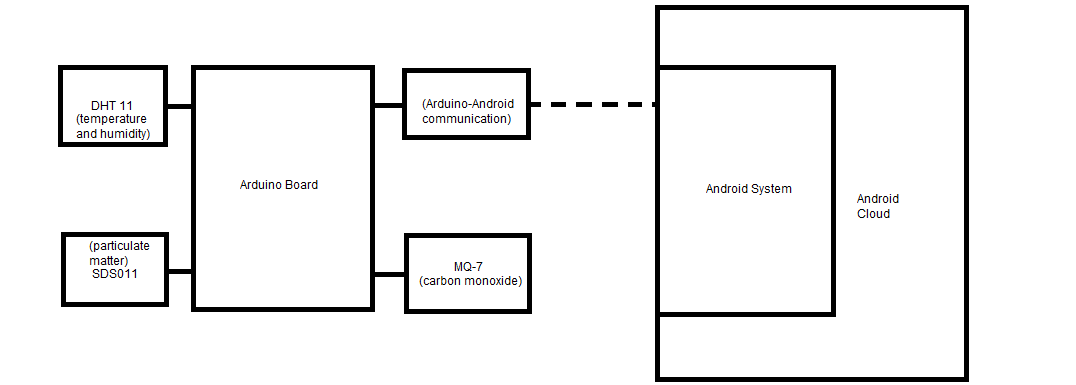
\includegraphics[width=\textwidth]{BlockDiagram}

\begin{center}
Figure 4.1. System Model of the Project
\end{center}

\begin{center}
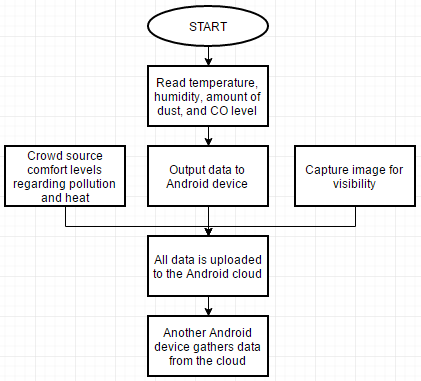
\includegraphics{Flowchart}
\end{center}




\begin{center}
Figure 4.2. System Flowchart
\end{center}

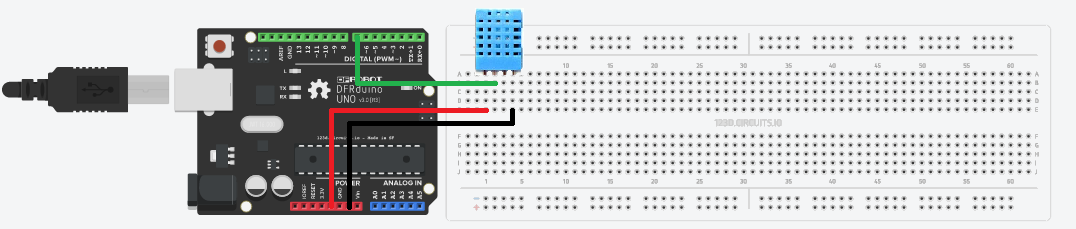
\includegraphics[width=\textwidth]{CurrentProgress}

\begin{center}
Figure 4.3. Circuit Configuration for Testing the DHT-11
\end{center}







\begin{lstlisting}
#include <dht.h>

dht DHT;

#define DHT11_PIN 7

void setup(){
  Serial.begin(9600);
}

void loop()
{
  int chk = DHT.read11(DHT11_PIN);
  Serial.print("Temperature = ");
  Serial.println(DHT.temperature);
  Serial.print("Humidity = ");
  Serial.println(DHT.humidity);
  delay(1000);
}
\end{lstlisting}

\begin{center}
Figure 4.4. Code for Temperature and Humidity Gathering
\end{center}
\begin{center}
\begin{eqnarray}
DI = T-0.55(1-0.01H)(T-14.5)
\label{Discomfort Index}
\end{eqnarray}
\end{center}
\begin{center}
Figure 4.5. Formula for Discomfort Index
\end{center}

\section{Summary}

According to the system model, the project will make use of an Arduino microcontroller system that will handle tasks of gathering inputs which are the temperature, humidity, amount of dust, and amount of carbon monoxide. These data will be transmitted an Android system. Afterwards, this data can be submitted  to the Android cloud in real time. Each individual Android system in the cloud can make use of the camera to capture the image of the surroundings in order to get the visibility with the aid of computer vision. A crowdsourcing element is considered to be added in each system where the user can rank the amount of discomfort he feels in terms of the heat and air pollution. This information will be utilized in the cloud.

The current accomplishments for the group is the successful gathering of the temperature and humidity with the use of the Arduino system and the DHT-11 sensor. These values are rounded to the nearest units value.